\documentclass[11pt]{article}

\usepackage{exscale}
\usepackage{graphicx}
\usepackage{amsmath}
\usepackage{latexsym}
\usepackage{times,mathptm}
\usepackage{epsfig}
\usepackage{setspace}

\textwidth 6.5truein          
\textheight 9.0truein
\oddsidemargin 0.0in
\topmargin -0.6in

\parindent 0pt          
\parskip 5pt
\def\baselinestretch{1.1}

\begin{document}

\begin{LARGE}
\centerline {\bf CSci 423 Homework 2}
\end{LARGE}
\vskip 0.25cm

\centerline{Due: 1:00 pm, Wednesday, 9/19}
\centerline{Eric Shih}

\begin{enumerate}

  \item (5 points) Give the state diagram of an NFA that recognizes the set of strings such that there are at lease 
  two 0s separated by a number of positions that is a multiple of 4. Note that 0 (as a number) is a multiple of 4.
  \begin{center}
    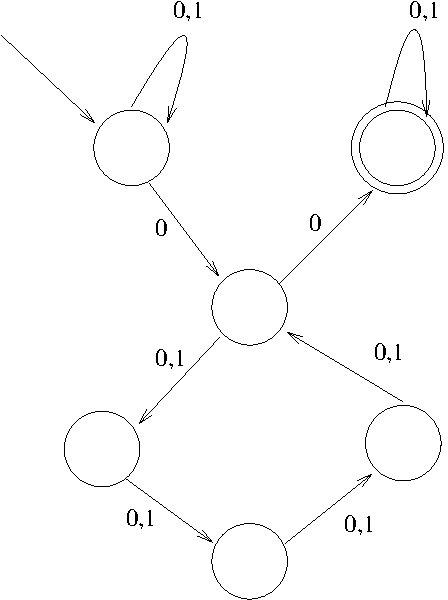
\includegraphics[scale=.4] {fig1.pdf}
  \end{center}
  
  \item (10 points) Exercise 1.7 (c) on page 84 and then convert the NFA to an equivalent DFA.
  \begin{center}
    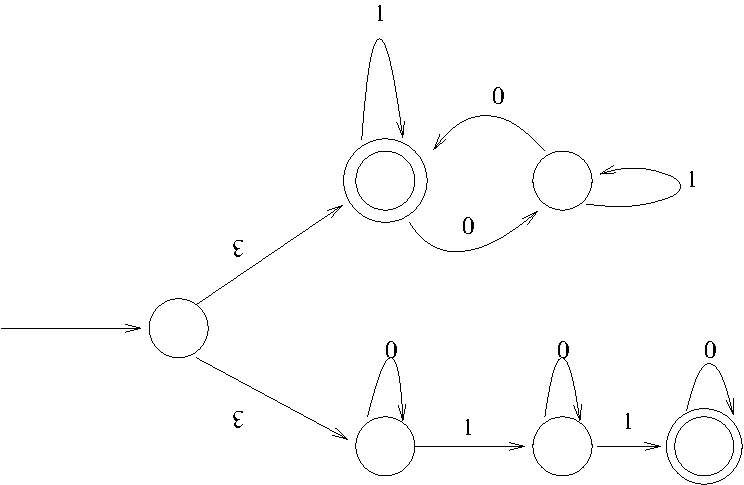
\includegraphics[scale=.4] {fig2.pdf} \\
     NFA \\
    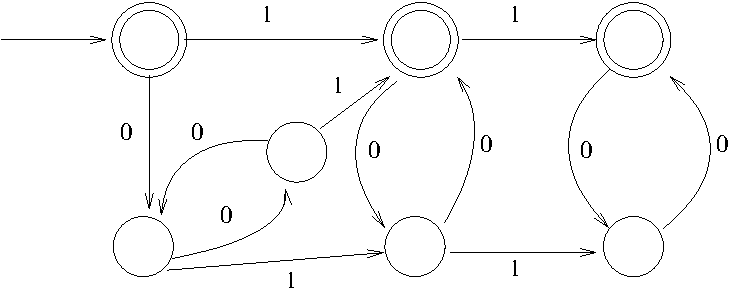
\includegraphics[scale=.4]{fig3.pdf} \\
     DFA
   \end{center}

  \item (10 points) Exercise 1.16 (b) on page 86 and then describe in a concise sentence the language recognized by 
  the FA.
  \begin{center}
    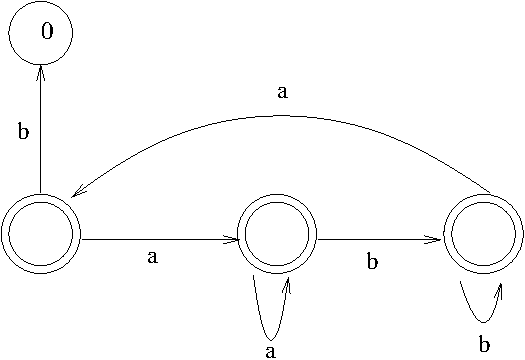
\includegraphics[scale=.4] {fig4.pdf} \\
    0 denotes null state
  \end{center}  

  \item(10 points) Problem 1.32 on page 88. \\
  \begin{center}
    Let a = $\begin{bmatrix} 0 \\ 0 \\ 0 \\ \end{bmatrix}$, b = $\begin{bmatrix} 0 \\ 0 \\ 1 \\ \end{bmatrix}$,
    c = $\begin{bmatrix} 0 \\ 1 \\ 0 \\ \end{bmatrix}$, d = $\begin{bmatrix} 0 \\ 1 \\ 1 \\ \end{bmatrix}$,
    e = $\begin{bmatrix} 1 \\ 0 \\ 0 \\ \end{bmatrix}$, f = $\begin{bmatrix} 1 \\ 0 \\ 1 \\ \end{bmatrix}$,
    g = $\begin{bmatrix} 1 \\ 1 \\ 0 \\ \end{bmatrix}$, h = $\begin{bmatrix} 1 \\ 1 \\ 1 \\ \end{bmatrix}$ \\
  \end{center}
  \begin{center}
    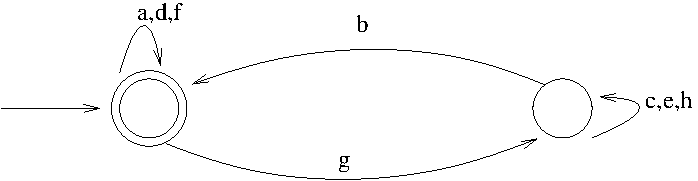
\includegraphics[scale=.4] {fig5.pdf}
  \end{center} 

  \item (5 points) For language L, let min(L)={w|w is in L but no proper prefix of w is in L}. Prove that if L is a 
  regular language, so is min(L). \\ *berkley.edu was used as an reference in this problem*\\
  If L is regular, there is a DFA that will accept it. If all outgoing edges in the accepting states of the DFA 
  print to a dead state, then the result is the DFA for $min(L)$. The new DFA is proven because anything accepted
  by the old DFA is still accepted except for anything that would pass through an accepting state. This property
  translates to $min(L)$, therefore proving that a DFA can be created and is a regular language.
\end{enumerate}

\pagebreak
\setlength{\parindent}{1cm}
\centerline{\bf Reading Summary 1}

\begin{spacing}{1.5}
\indent The common problem in online text repositories is that with a given set of words, we need to find all documents
that contain those words. To solve this problem, many search engines use inverted indexes. Inverted indexes solves the
problem by storing a list of all the places where the word occurs for each word. This amounts to a gigantic amount
of memory used. To populate this list, crawlers are used to go through the web. These crawlers do not use finite
automata. The applications that are suitable for automata searches generally have a repository that is rapidly 
changing and cannot be cataloged. Good examples of a rapidly changing repository are stock ticker information and
a goods catalog that retrieves up-to-date prices. An example of applications that cannot be cataloged is query 
responses that generate responses as the request is made. \\
\indent Nondeterministic finite automation can be used to deal with keywords and finding any occurrences of this
set of words. Using the nondeterministic finite automation will use an accepting state to signal when a keyword
has been hit. This process requires that the word is fed into the NFA one character at a time. The simple process
of recognizing a key word consists of a start state with transitions to itself for every input symbol and a state
for every keyword that is connected by the appropriate symbol as a transition between the states. The example given
in the article describes an NFA that needs to recognize the words ``web'' and ``eBay''. The two choices to implement
the NFA are to have a program that computes the set of states after reading each input symbo, or to convert the NFA
to a DFA and then simulate the DFA. For this example, the DFA conversion was the easiest option. \\
\indent The number of states in the DFA when doing the subset construction for keywords will never be greater than
the number of states in the NFA. This worst case scenario is a big reason why DFA conversion is used often. To
construct the DFA a few rules must be followed. First if $q_0$ is the start state of the NFA, then ${q_0}$ is one
of the states of the DFA. Then the DFA states must consist of $q_0$, the state in focus from the NFA, and every
other state in the NFA that is reachable from $q_0$. Usually the states will match up directly, but sometimes two
states will yield the same NFA states, and combine to become one DFA state.
\end{spacing}

\end{document}
